% $Id$

Chapter \ref{ch:findchirp} described the algorithms that we use to generate
inspiral triggers given an inspiral template and a single data segment.
There is more to searching for gravitational waves from binary inspiral than
trigger generation, however. To perform a search for a given class of sources in a
large quantity of interferometer data we construct a \emph{detection
pipeline}.  In section \ref{s:construction} we give an overview of the
the components used in a pipeline and how they fit together.
We then describe the building blocks of the pipeline in more detail. Section
\ref{s:dq} describes data quality cuts, which are used to discard unstable
data. The application of trigger generation to the data is explained in
section \ref{s:pipetemplate}. The use of data from multiple interferometers is
decribed in section \ref{s:coincidence}. In section \ref{s:vetoes} we
show how data from the interferometer that does not measure the gravitational
wave signal can be used.  Finally in section \ref{s:s2pipeline} we describe
the pipeline that has been constructed to search for binary neutron stars and
binary black hole MACHOs in the S2 data.

\section{Construction of Inspiral Pipelines}
\label{s:construction}

A detection pipeline is a sequence of operations that starts with the raw data
from the interferometers and produces a list of \emph{candidate events}.
Figure \ref{f:simple_pipe} shows a simple pipeline to filter the data from a
pair of interferometers labeled IFO$1$ and IFO$2$.
We first consider the data from the interferometers. In order to analyze
data, it must come from interferometers in stable operation. Running an
interferometer is a complex process that requires \emph{operators} trained to
align and lock the interferometers and to monitor the quality of the data
being taken. From a quiescent state, the operators manually align the optics
of the interferometer to within appropriate parameters. The operators then
direct the automated length sensing and control system to bring the
Fabry--Perot cavities into resonance; the beam splitter is positioned so that
the light at the anti-symmetric port is a minimum. The recycling cavity is
then brought into resonance and an automated script reports to the operators
that the interferometer is \emph{locked}. In addition to the operator, 
members of the LIGO Scientific Collaboration trained in the operation
of the interferometer are present at the observatory. The collaboration member
on duty is known as the as scientific monitor or \emph{scimon}. Once the
interferometer is locked, the operator and scimon decide if the quality of the
data being recorded is suitable to be flagged as \emph{science mode data}. If 
the data is suitable it is then used for gravitational wave analysis.

It is possible that the operators or scimons may make mistakes in deciding
that data should be flagged as science mode; they may forget to enable
calibration lines, for example. There may also be noise sources or transient
events in the data which make it unsuitable for analysis but which are not
easily detectable in the control room while the data is being taken. To
prevent such data from being using in an astrophysical analysis several
\emph{data quality cuts} are used to discard poor quality data. The manual
selection of science mode data may be considered as the first data quality
cut.  Additional tests if data quality are described in section \ref{s:dq}.

The matched filtering described in the previous chapter generates triggers for
a single inspiral template. We generally wish to search the data for a class
of signals. In this thesis, we describe searching for gravitational waves from
binary neutron stars and binary black hole MACHOs.  Both sources use the
second order post-Newtonian stationary phase templates described in chapter
\ref{ch:inspiral} and the search algorithms described in chapter
\ref{ch:findchirp}. The inspiral signals from a class of sources will lie in
some region of the template parameter space described by the component masses
$m_1$ and $m_2$. This means that a single template is not sufficent to search
for signals from the population, as template for a given pair of mass
parameters may not produce a hight signal-to-noise ratio when used to filter a
signal with different mass parameters. To search a region in parameter space
we construct a \emph{bank} of inspiral templates as described in section
\ref{s:pipetemplate}. The template bank is constructed to cover the parameter
space in such a way that we do not discard any signals from our target
population.

We then use the template bank to filter the data for inspiral signals using
the matched filter and $\chi^2$ veto. This generates a list of \emph{inspiral
triggers} for each interferometer. In the pipeline shown in figure
\ref{f:simple_pipe} a template bank is generated for each interferometer and
the data from an interferometer filtered through the bank particular to that
data. Section \ref{s:pipetemplate} describes in more detail how trigger
generation is used in a pipeline.

One of the most powerful methods of rejecting false alarms is coincidence
between different interferometers. As described previously, there are three
LIGO interferometers which are operated simultaneously during science runs.
The interferometers are named H1, H2 and L1. The H1 and H2 detectors are
$4$~km and $2$~km long interferometers, respectively, co-located to the LIGO
Hanford Observatory. The L1 detector is a $4$~km long interferometer located
at the LIGO Livingston Observatory. A true gravitational wave should be found
in all operating detectors at the same time, up to the error in measurement of
arrival time and the time it takes a gravitational wave to propagate between
the observatories. This
\emph{time coincidence} test can be applied to inspiral triggers from each
interferometer and is an excellent method of distinguishing real signals from
noise. Other coincidence tests may be used, such as demanding consistency of
the waveform parameters between triggers from two detectors, or consistency in
the recovered amplitude of the signal relative to the sensitivity of the
detectors. We describe these tests in section \ref{s:coincidence}.

While the goal of the interferometer commissioners and operators is to ensure
that the data recorded is as stationary and Gaussian as possible, transient
noise sources may still be present in the data. For example it has been seen
that a person jumping up and down in the control room at the observatory will
cause a burst of noise in the gravitational wave channel. There may also be
occasional glitches in the interferometer control systems that cause a
transient in the gravitational wave channel, despite the best efforts of the
experimental team. To allow us to distinguish such events from true
gravitational wave signals, we record several thousand data streams of
auxiliary interferometer control channels and physical environment monitor
(PEM) channels. Auxiliary channels monitor the state of the servo loops that
control the interferometer and include information about the pre-stabilized
laser, the length sensing and control system and the input and output optics.
PEM channels record the data from devices such as seismometers, magnetometers
and microphones placed in and around the interferometer. These devices are
designed to detect environmental sources that may couple to signals in the
gravitational wave channel. This data can be used to construct \emph{vetoes}
on the inspiral triggers if a coupling can be identified between a noise
source present in an auxiliary or PEM channel and inspiral triggers in the
gravitational wave channel.  We demonstrate this process with examples in
section \ref{s:vetoes}. 

The final step in constructing a pipeline is to turn the chosen algorithm into
code that can be executed in an automated way on a computing cluster. The
execution of the code must ensures that all the input data has been analyzed
and the components of the pipeline are executed in the correct sequence. To do
this we construct a directed acyclic graph (DAG) that describes the work flow
for the pipeline.  For example, we may construct write a DAG to execute the
simple pipeline in figure \ref{f:simple_pipe} on all the data from L1 and H1
recorded in S2. The DAG describing the work flow is submitted to a computing
cluster via the Condor high throughput computing system. The Condor DAG
manager executes the pipeline described in the. This process is described in
more detail in section \ref{s:dag}.

Implicit in the above discussion is that fact that there are many parameters
that must be set at each stage of the pipeline. For example: What data quality
cuts should we use? What signal-to-noise and $\chi^2$ thresholds should we use
when generating the inspiral triggers? What coincidence tests should we apply
and what should their parameters be? What auxiliary channels and PEM channels
should be used and vetoes and how do we apply the vetoes that we choose to
inspiral triggers? Answering these questions is the key to turning a pipeline
into a full binary inspiral search; we call the process of selecting the
parameters \emph{tuning the pipeline}. In fact, pipeline tuning and
construction of the pipeline are not entirely separate. After constructing a
pipeline and initial tuning, we may decide to revisit the pipeline algorithm
before performing additional tuning.

When tuning the pipeline we may wish to minimize the \emph{false alarm rate},
i.e. minimize the number of candidate events that are not due to inspiral
signals.  We may also wish to minimize the false dismissal rate to ensure that
the pipeline does not discard triggers that are due to real signals.  False
alarm rate can be studied by looking at candidate events in the playground and
false dismissal rate can be studied by \emph{injecting} signals into the data,
that is generating a known inspiral signal and adding it to the data before
passing it through the pipeline. Injection of signals is described in section
\ref{s:eff} and chapter \ref{ch:hardware}.

When tuning the pipeline for data that will be used to produce an upper limit,
we must ensure that we do not introduce statistical bias. To do this, we
select $10\%$ of all the data that we record as \emph{playground data}. The
data from GPS time $[t,t+1)$ is playground if 
\begin{equation}
t - 729273613 < 600 \quad \mathrm{mod}(6370).
\end{equation}
Playground data is selected algorithmically to provide a representative sample
of the full data set. We are free to pursue whatever investigations that we
wish on the playground data. We do not use this data in the upper limit
calculation, however we do not preclude the detection of a gravitational wave
signal in this data. We describe the process of tuning the S2 binary neutron
star search in chapter \ref{ch:bns} and the S2 binary black hole MACHO search
in chapter \ref{ch:result}.

If we are using data from multiple interferometers we can measure the
\emph{background rate} of inspiral signals. We do this by introducing a time
shift into the data from different detectors before passing it through the
pipeline. If we assume that noise between the detectors is uncorrelated and
the time shift is sufficiently large, as described in section
\ref{s:background}, then any candidate events that survive the pipeline should
be due to noise alone and not astrophysical signals. By measuring the
background rate, we can measure the false alarm rate of the pipeline which can
be used for both tuning and the computation of the upper limit or detection
confidence.

\section{Data Quality Cuts}
\label{s:dq}

The theoretical matched filter is optimized for data with a known, calibrated
noise spectrum which is stationary over the time scale of the data analyzed.
This requires stable, well-characterized interferometer performance. In practice,
the interferometer performance is influenced by optical alignment, servo
control settings, and environmental conditions. The list of science mode data
provided by the operators can contain times when the interferometer is not
operating correctly. Unstable interferometer data can produce false triggers
that may survive both the $\chi^2$ test and coincidence.  Data quality cuts
evaluate the interferometer data over relatively long time intervals, using
several different tests, or look for specific behaviour in the interferometer
to exclude science mode data that is unsuitable for analysis.  To decide if we
should exclude science mode data based on a particular data quality cut, we
can examine the performance of the inspiral code on data which is flagged as
suspect by the cut. In this sections \ref{ss:photodiode} and \ref{ss:calcut}
we illustrate the motivation for data quality cuts with two examples. In
section \ref{ss:s2dq} we list the data quality cuts cuts available in S2.
Section \ref{ss:s2dqselection} discusses how the final selection was chosen for
the S2 BNS and BBHMACHO pipelines.

\subsection{Photodiode Saturation}
\label{ss:photodiode}

Figure \ref{f:s1loudest} shows the signal-to-noise ratio and $\chi^2$ time
series of the loudest candidate event that was produced by the LIGO S1
inspiral search. Also shown is the filter output for an inspiral waveform with
similar parameters that is injected into the well behaved interferometer data.
Notice that the time series of $\rho(t)$, $\chi^2(t)$ and the raw data are
very noisy around the time of the S1 loudest candidate. In contrast, the time
series for the simulated signal is very clean. On further investigation, we
determined that at the time of the S1 loudest event, the photodiode that
records the light at the anti-symmertic port has saturated. The system that
converts the light into an electronic signal for the length sensing an control
servo had exceeded its dynamic range causing a noise transient in the data.
As well as the saturation itself being problematic, it was determined that
saturation is a symptom of poor interferometer performance. Photodiode
saturations are caused by large bursts of noise in the gravity wave channel
which corrupt power spectral estimation and matched filtering. A test was
developed to monitor the gravity wave channel for photodiode saturations and
this test has become a data quality cut for current and future searches.

\subsection{Calibration Lines}
\label{ss:calcut}

A second example of a data quality cut is the presence of calibration lines,
which were described in section \ref{ss:calibration}. The calibration lines
track the response of the instrument to a gravitational wave, which varies
over time and without the calibration lines present, it is not possible to
construct a satisfactory response function. Since the inspiral search needs
correctly calibrated data, a simple data quality cut checks for the presence
of the calibration lines in the data. If they are absent the data is
discarded.

\subsection{Data Quality Cuts Avaliable in S2}
\label{ss:s2dq}

The full list of avaliable data quality cuts and their meanings for S2 are
show in table \ref{t:dqflags}. The table is divided into two sections,
mandatory and discretionary data quality cuts. Mandatory cuts represent
unrecoverable problems in data aquisition or calibration and so we must exlude
these times from the list of science mode segments. Discretionary data cuts
are optional for a particular search. For the inspiral search we can decide
whether or not to use a cut based on the performance of the trigger generation
code in playground data when a particular data quality cut is active, as
described in section \ref{ss:s2dqselection}.

\section{Inspiral Trigger Generation}
\label{s:pipetemplate}

Chapter \ref{ch:findchirp} describes the algorithms that we use to determine
if an inspiral from a binary of masses ${m_1,m_2}$ is present in a single data
segment. The input to trigger generation is \emph{(i)} the template,
$\tilde{h}_{ck}$, \emph{(ii)} the data segment to be filtered, $\{v_j\} j \in
[0,N]$, \emph(iv) an average power spectral density, $\ospsd$, which measures
the noise in the interferometer and \emph{(iv)} the instrumental response
function, $R(f)$, which is required to calibrate the data. We have described
how we select the data to be filtered by applying data quality cuts to science
mode data. The times remaining after we apply data quality cuts are called
\emph{science segments}. Section \ref{ss:datamanagement} decribes how we
obtain data segments, power spectra and response functions from the science
segments. We then describe the process of template bank generation in section
\ref{ss:templatebank} and finally enumerate the various parameters that can be
tuned for inspiral trigger generation in section \ref{ss:triggerparameters}.

\subsection{Data Management}
\label{ss:datamanagement}

Corruption to to wraparound of the matched filter means that not all the time
in a data segment can be searched for triggers. As mentioned in chapter
\ref{ch:findchirp}, we simplify the process of selecting uncorrupted data by
only searching for triggers in the signal-to-noise ratio, $\rho^2(t_j)$, when 
\begin{equation}
\frac{N}{4} \le j < \frac{4N}{4},
\end{equation}
where $N$ is the number of sample points in the data segment, and demanding
that the amount of data corrupted is less than $N/4$ sample points. To ensure
that all data is analyzed we must overlap each data segment by $(N/2)\Deltat
t$~seconds. To compute an average power spectrum we require a sample of data
near the data segment being filtered so that a good estimate of the noise can
be obtained; the power spectral estimate also requires overlapping data
segments. We combine these two requirements by bundling several overlapping
data segments together in an \emph{analysis chunk}. The length of an analysis
chunk is bounded above by the amount of memory avaliable in the computers
performing the filtering and bounded below by required a sufficently large
number of segments in the computation of the average power spectrum. In S2, we
constructed analysis chunks of length $2048$~seconds from $15$ data segments
of length $256$~seconds. The data segments are overlapped by $128$~seconds,
with the first and last $64$ seconds of data segment ignored when searching
for triggers. 

The interferometer records data at $16\,384$~Hz, so we downsample the analysis
chunk to a sample rate of $4096$~Hz after reading it from disk to decrease the
computational resources required by the filtering code.  We do this by
applying a finite impulse response (FIR) low pass filter to remove power above
the Nyquist frequncy of the desired sample rate, $2048$~Hz. The low passed
data is then decimated the to the desired sample rate. The highest frequency
of gravitational radiation we are filtering in the binary neutron star is
$\sim 2080$~Hz, so we do not lose signal to noise ratio due to the lower
Nyqist frequency. The maximum frequency of most of the MACHO signals is
greater than $2048$~Hz and so we do lose some signal-to-noise ratio by
resampling. We can neglect this loss, however, becuase most of the
signal-to-noise is accumulated at frequencies lower than $2048$~Hz, as
described in chapter \ref{ch:inspiral}. Figure \ref{f:macho_snr_loss} shows
the loss in signal-to-noise ratio in the worst case for MACHO binary search.
The inspiral waveform of a pair of $0.2\,M_\odot$ black holes an effective
distance of $25$~kpcis generated at a sample rate of $16\,384$~Hz. The maximum
frequency of this waveform is $10\,112$~Hz. The waveform is injected into raw
(un-resampled) data with a typical S2 noise curve which is then filtered at
$16\,384$~Hz and $4096$~Hz. The maximum of the signal-to-noise ratio is $\rho
= 73.67$ for the raw data and $\rho = 73.58$ for the resampled data, giving a
difference in signal-to-noise ratio of $0.1\%$. The MACHO search is much more
compulationally intensive than the binary neutron star search, for reasons
explained in the next section, so this small loss of signal-to-noise is
greatly outweighed by gains in computational efficency due to resampling.

The interferometer data contains a large amount of power of seismic origin at
low frequencies.  This power is several orders of magnitude higher than the
noise in the sensitive frequency band of the interferometer. This amplitude of
the siesmic noise is sufficently large to overwhelm the windowing used to
prevent power in the power spectral estimation from bleeding into adjacent
bins. In order to remove this noise, we apply an infinite impulse response
(IIR) high pass filter to the resampled data. The high pass frequency and
filter order are chosen so that power in the sensitive band of the
interferometer is not attenuated. We also apply a low frequency cutoff in the
time domain. The matched filter correlation is not computed below this
frequency.

A windowed copy of each of the $15$ data segment is used to construct the
average power spectral density used in the matched filter, as described in
section \ref{s:psd}. Note that the data used in the matched filter is not
windowed; the windowed data is discarded once it has been used to compute the
power spectra.  The mean values over the analysis chunk of the calibration
parameters $\alpha$ and $\beta$ are used to construct the response $R(f)$. The
same response function is used to the power spectral density and all data
segments in the chunk.  Figure \ref{f:s2_segments} shows how analysis chunks
are constructed from the science segments in S2. The first analysis chunk is
aligned with the start of the science segment. Subsequent chunks overlap the
previous one by $128$~seconds. At the end of a science segment there is
generally not enough data to fit an entire analysis chunk but we cannot make
the chunk shorted, as we need all $15$ data segments to compute the average
power spectrum. To solve this problem, we align the end of the last chunk with
the end of the science segment and ignore any inspiral triggers generated for
times that overlap the previous chunk. 

A disadvantage to the above method of processing the input data is that we
require a science segment to be at least $2048$~seconds long. Any shorted
science segments are ignored, as there is not enough data to generate a power
spectral density. We note here that this lead to a significant amount of data
being discarded in the S2 analysis. As we will describe below, the S2 pipeline
requires the L1 interferometer to be operating in order to analyze the data.
L1 is the least stable of the inteferometers as it is very sensitive to
seismic noise. High seismic noise can saturate the length sensing and control
servo and cause the loss of lock, which terminates a science segment.
Modification of the filtering to overcome this limitation requires significant
changes of the implementation of the filtering code. It was not possible to
implement and test these changes within the time allowed to perform the S2
analysis. Fortunately, it is expected that after the installation of addition
seismic isolation at the Livingston observatory after the S3, the lengths of
science segments will be significantly improved, so the number of short
segments discarded will decrease. Unfortuatly S3 data exhibits the
problem of short science segments, so a redesign of the filtering code may
still be required.

\subsection{Template Banks}
\label{ss:templatebank}

We wish to use matched filtering and the $\chi^2$ veto to detect the inspiral
waveforms from binary neutron stars in the mass range $1\,M_\odot\le m_1,
m_2\le 3\,M_\odot$ and binary black hole MACHOs in the mass range
$0.2\,M_\odot\le m_2, m_1\le 1\,M_\odot$. Each mass pair $\{m_1,m_2\}$
produces a slightly different waveform. If we only used a single template to
search for inspiral waveforms, then the correlation of 


, we constructed a {\em bank} of
templates to filter the data. The template bank 


with different mass pairs such that, for any actual mass pair in the
parameter space of interest the loss of SNR due to the mismatch of the true
waveform from that of the best fitting waveform from the bank is less than
$3\%$ in the case of binary neutron stars and $5\%$ in the case of
BBHMACHOs\cite{owensatyha}.  The size of the template bank depends on the
shape (but not overall scale) of the power spectral density of the
interferometer and the mass parameter space. Due to to the chirp nature of
inspiral signals there are more cycles in the chirp at lower frequencies. In
addition, low mass signals produce longer chirps with more cycles in the
sensitive band of the detector. An interferometer with good low frequency
sensitivity y will require more templates then one with poorer low frequency
sensitivity as the matched filter will be more sensitive to the low frequency
part of the chirp. A bank that covers a lower mass inspiral signals will be
bigger than a higher mass bank due to the longer length of the low mass signals. 
Typical numbers for the size of the template banks for the Livingston 4km
interferometer are $900$ for binary neutron starts and $14\,000$ for binary
black hole MACHOs.

The input to the inspiral trigger generation algorithm is an inspiral
template, a finite stretch of interferometer data, an average power spectral
estimate of the noise in the input data and a instrument response function
describing the response of the interferometer to gravitational waves as a
function of frequency. This input is constructed from the interferometer data
as follows.  

The interferometer operators, in consultation with scientific monitors present
at the observatory during data taking, flag times when the interferometers are
in stable operation and the data is suitable for analysis.  Times when an
interferometer was in stable operation are identified as ``science segments''.
These science segments were analyzed in ``analysis chunks'' of 2048 seconds.
The length of the analysis chunks are chosen based on the available memory in
the hardware used to perform the search.  The analysis chunks are further
divided into data segments of length $256$ seconds. The length of the data
segment is set by the length of the longest chirp in the template bank and the
length of the square root of the inverse power spectrum in the time domain,
which must be shorter than one quarter of a segment.  Triggers are not
generated for the first and last $64$~s of a given data segment due to wrap
around, so we overlap subsequent data segments by $128$~s to ensure that all
data is filtered for triggers. Therefore there are $15$ data segments in an
analysis chunk. Since the first and last $64$ seconds of a chunk are not
analyzed, the chunks are also overlapped by $128$ seconds.  If a science
segment cannot be exactly divided into overlapping chunks (as is usually the
case) the remainder of the data is covered by a special $2048$-s chunk which
overlaps with the previous chunk as much as necessary to allow it to end at
the end of the segment.  For this final chunk, a parameter was set to restrict
the inspiral search to the time interval not covered by any other chunk. 

  The
power spectrum $S_n(f)$ for the $2048$ seconds of data was estimated by taking
the median of the power spectra of the $15$ segments.  The calibration,
$R(f)$, was generated for each chunk using the mean value of the calibration
factors $\alpha$ and $\beta$ over the chunk.  The algorithm to construct the
filter input from the science segments is shown in figure~\ref{f:s2_segments}.

For a given template multiple triggers can be recorded in a segment.  The
triggers are clustered so that distinct triggers are separated by at least the
length of the template.  Each analysis segment is filtered through all the
templates. It is possible for multiple templates to trigger at same time.

\subsection{Trigger Generation Parameters}
\label{ss:triggerparameters}

To summarize: for a given template we use matched
filtering to construct the signal-to-noise ratio, $\rho$, and search for times
when this exceeds a threshold, $\rho > \rho^\ast$. If this happens, we
construct a template based veto, the $\chi^2$ veto\cite{brucechisq}. Small
values of $\chi^2$ indicate that the signal-to-noise was accumulated in a
manner consistent with an inspiral signal. If the value of the $\chi^2$ veto
is below a threshold, $\chi^2 < {\chi^2}^\ast$, then an inspiral trigger is
recorded at the maximum value of $\rho$.


\section{Trigger Coincidence}
\label{s:coincidence}

The time difference between gravitational wave arrival time
may be between $0$~seconds, if the gravitational wave is propagating
perpendicular to a line joining the detectors, or $10$~ms if the gravitational
wave is propagating parallel to a line joining the detectors. The maximum
time difference comes from the time it takes a gravitational wave to propagate
between the observatories, given by $t = \frac{d}{c}$, where $d = x$~km is the
distance between the observatories and $c$ is the speed of light.


For a trigger to be considered coincident in two interferometers, we demand
that it is observed in both interferometers within a temporal coincidence
window, $\delta t$, that allows for the error in measurement of the time of
the trigger. Monte Carlo analysis with simulated signals suggests that we
cannot measure the time of the trigger to an accuracy of less than $1$~ms, so
we demand $\delta t = 1$~ms if the interferometers are located at the same
observatory. If the detectors are not co-located, we allow for the $10$~ms
light travel time between the LIGO observatories by demanding $\delta t =
11$~ms. We also demand that the waveform of the triggers are consistent by
requiring that the two mass parameters, $m_1$ and $m_2$, of the binary are
identical to within an error of $\delta m$.

We now consider an amplitude cut on the signals. The Livingston and Hanford
detectors are not co-aligned. There is a slight misalignment of the detectors
due to the curvature of the earth and so the antenna patterns of the detectors
differ. This causes the measured amplitude of a gravitational wave to differ
between the sites. In the extreme case, it is possible for a binary to be
completely undetectable by the L1 detector, but still detectable by the H1 and
H2 detectors. For a given inspiral trigger, we measure the \emph{effective
distance} of the binary system. This is the distance at which an optimally
oriented binary would produce the observed signal-to-noise ratio.
Figure~\ref{f:gmst_dist_ratio} shows the ratio of effective distances between
the two LIGO observatories for the population of binary neutron stars
considered in the S2 analysis. The significant variation of the effective
distance precludes using a naive test for amplitude coincidence. It is
possible to obtain information about sky position from time delay between
sites to construct a more complicated amplitude cut, but this has not be used
in the S2 analysis.

In the case of triggers from the H1 and H2 interferometers that are coincident
in time and mass, we apply an amplitude cut that tests that the effective
distance of the triggers is coincident given the relative sensitivity of the
detectors, while allowing for error in this measurement which is determined by
Monte Carlo simulations.  When testing for triple coincident triggers we 
accept triggers that are coincident in the L1 and H1 detectors that are
\emph{not} present in the H2 detector \emph{if} the effective distance of the
trigger is further than the maximum distance of H2 at signal-to-noise ratio
$6$ at the time of the candidate trigger. Figure \ref{f:coinc_test} summarizes
the time, mass and distance coincidence test.  The final step of the pipeline
is to apply and auxiliary interferometer vetoes described in
section~\ref{s:vetoes}. 

The list of surviving candidate triggers is followed up by examining the raw
gravitational wave data, auxiliary interferometer channels and physical
environment monitoring channels to determine if the triggers are truly of
astrophysical origin.


\section{Auxiliary and Environmental Channel Vetoes}
\label{s:vetoes}

The other method was to look for signatures in environmental monitoring
channels and auxiliary interferometer channels which would indicate an
external disturbance or instrumental ``glitch'', allowing us to {\it veto} any
triggers recorded at that time.

Auxiliary interferometer channels (which monitor the light in the
interferometer at points other than the antisymmetric port---where a
gravitational wave would be most evident) were examined, with the aim being to
look for correlations between glitches found in the readouts of these channels
and inspiral event triggers found in the playground data.  By doing so, we are
capable of identifying instrumental artifacts that directly affect the light
that is measured in the gravitational wave channel, so these vetoes are
potentially very powerful.  However, we had to consider the possibility that a
gravitational wave itself could produce the observed glitches in the auxiliary
channel due to some physical or electronic coupling.  This possibility was
tested by means of {\em hardware} injections, in which a simulated inspiral
signal is injected into the interferometer by physically moving one of the end
mirrors of the interferometer. Hardware injections allow us to establish a
limit on the effect that a true signal would have on the auxiliary channels.
Only those channels that were unaffected by the hardware injections were
considered ``safe'' for use as potential veto channels. Hardware injections
are described in more detail in chapter \ref{ch:hardware}.

We used a computer program, {\it glitchMon} \cite{glitchMon}, to examine the
data and identify large amplitude transient signals in auxiliary channels.
Numerous channels, with various filters and threshold settings, were examined
with glitchMon. The program produces a list of times when the glitches
occurred. The glitch event list was compared with times generated by triggers
from the inspiral search; all of these preliminary studies were conducted on
the playground data. A time window around a glitch was defined, and any
inspiral event within this window was rejected. One can associate the veto
with inspiral event candidates and evaluate a veto efficiency (percentage of
inspiral events eliminated), use percentage (percentage of veto triggers which
veto at least one inspiral event), and dead-time (percentage of science-data
time eliminated by the veto). The results of the veto investigations for
binary neutron stars are described in section \ref{s:} and for binary black
hole MACHOs in section \ref{s:}.

During investigation of inspiral triggers in the playground data, it was
discovered that many of the L1 inspiral triggers appeared to be the result of
non-stationary noise with frequency content around $70$~Hz.  An important
auxiliary channel, \texttt{L1:LSC-POB\_I}, proportional to the residual length
of the power recycling cavity, was found to have highly variable noise at
$70$~Hz.  There are understandable physical reasons for this, namely the power
recycling servo loop (for which \texttt{L1:LSC-POB\_I} is the error signal)
has a known instability around $70$~Hz, which often results in the appearance
of glitches in the detector output channel at around $70$~Hz.  As a
consequence, it was decided that the low-frequency cutoff of the binary
neutron star inspiral search should be set to $100$~Hz to reduce sensitivity
to these glitches.  This subsequently reduced the number of inspiral triggers
(presumably created by this problem); an inspection of artificial signals
injected into the interferometer revealed a very small loss of efficiency for
binary neutron star inspiral and BBHMACHO signal detection resulting from the
increase in the low frequency cutoff.

\section{Directed Acyclic Graphs}
\label{s:dag}

\section{Background Estimation}
\label{s:background}

Since we restrict the S2 analysis to coincident data and require that at least
two of the interferometers must be located at different observatories, we may
measure a background rate for our analysis. After generating triggers for each
interferometer, we slide the triggers from one observatory relative to the
other observatory and look for coincidences between the shifted and zero lag
triggers. The minimum slide length is chosen to be greater than the length of
the longest filter ($20$~seconds) so any coincident triggers detected must be due to background and
not astrophysical events. By examining the distribution of background events
in the $(\rho_\mathrm{H},\rho_\mathrm{L})$ plane we can attempt to determine
contours of constant false alarm rate in order to construct a combined
effective signal-to-noise ratio for a coincident trigger\cite{abbott2004a}.

\section{Detection Efficiency}
\label{s:eff}

In absence of detection, we will construct an upper limit on event rate.  To
do this, need to measure the detection efficiency of the analysis pipeline to
our population. A Monte Carlo method is used to measure this efficiency. We
simulate a population of binary neutron stars and \emph{inject} signals from
that population into the data from all three LIGO interferometers. The
injection is performed in software by generating an inspiral waveform and
adding it to interferometer data immediately after the raw data is read from
disk. We inject the actual waveform that would be detected in a given
interferometer accounting for both the masses, orientation, polarization, sky
position and distance of the binary, the antenna pattern and calibration of
the interferometer into which this signal is injected.  The effectiveness of
software injections for measuring the response of the instrument to an
inspiral signal is validated against hardware injections where
an inspiral signal is added to the interferometer control servo during
operation to produce the same output signal as a real gravitational wave. This
validation is described in chapter \ref{ch:hardware}. The
data with injections is run through the full analysis pipeline to produce a
list of inspiral triggers. The detection efficiency of the pipeline,
$\epsilon$, is the ratio of the number of detected signals to the number of
injected signals.

\section{The S2 Data Analysis Pipeline}
\label{s:s2pipeline}

In this section we describe the pipeline constructed to search the S2 data for
gravitational waves from inspiralling binary neutron stars and binary black
hole MACHOs. The data quality cuts used are common to both searches and are
described in section \ref{ss:s2dqselection}. The detection of a
gravitational-wave inspiral signal in the S2 data would (at the least) require
triggers in both L1 and one or more of the Hanford instruments with consistent
arrival times (separated by less than the light travel time between the
detectors) and waveform parameters. During the S2 run, the three LIGO
detectors had substantially different sensitivities, as can be seen from
figure \ref{f:s2noisecurve}. The sensitivity of the L1 detector was greater
than those of the Hanford detectors throughout the run. Since the orientations
of the LIGO interferometers are similar, we expect that signals of
astrophysical origin detected in the Hanford interferometers are detectable in
the L1 interferometer.  We use this and the requirement that a signal be
detected in both the Livingston and at least one of the Hanford
interferometers to construct a {\em triggered search} pipeline. The
construction of this triggered search pipeline is described in section
\ref{ss:triggeredsearch}. Finally we describe a test of this pipeline in
section \ref{ss:triggeredtest}. Full details of tuning and the results of the
search for binary neutron stars and binary black hole MACHOs are presented in
the following chapters.

\subsection{Selection of Data Quality Cuts for S2}
\label{ss:s2dqselection}

Playground data from each of the three interferometers was analyzed separately
producing a list of inspiral triggers from each interferometer. Only the
mandatory data quality cuts were used to exclude time from the science mode
segments. Each interferometer was filtered separately using template banks
particular to that interferometer. No coincidence was applied between
interferometers; data quality cuts were tested independently on the three
lists of inspiral triggers produced. Table \ref{t:s2dqresults} shows the the
correlation of inspiral triggers with a particular data quality cut for
triggers of different signal to noise. When selecting the data quality cuts we
must be aware of three constraints. The first is that the data quality cuts
are based on data from the gravitational wave channel so it is important to
ensure that a data quality cut is not triggered by a real signal in the data.
For this reason we always use caution when selecting a cut base on noise in
AS\_Q.  The second constraint is to not exclude large amounts of data from the
analysis as the signals that we are looking for are rare. Finally we base our
choice on reccomendations from the experiemental team. They may decide that a
cut should be used, even if it does not correlate with inspiral triggers, as
any detection made in such a time could not be trusted. Table
\ref{t:s2dqchoice} shows the final choice of discretionary data quality cuts
and the reasons for them.

\subsection{A triggered search pipeline}
\label{ss:triggeredsearch}

During the S2 run, the three LIGO detectors had substantially different
sensitivities, as can be seen from figure \ref{f:s2noisecurve}. The
sensitivity of the L1 detector was greater than those of the Hanford detectors
throughout the run. Since the orientations of the LIGO interferometers are
similar, we expect that signals of astrophysical origin detected in the
Hanford interferometers are detectable in the L1 interferometer.  We use this
and the requirement that a signal be detected in both the Livingston and at
least one of the Hanford interferometers to construct a {\em triggered search}
pipeline, summarized in Fig.~\ref{f:pipeline}. We search for inspiral triggers
in the most sensitive interferometer (L1), and only when a trigger is found in
this interferometer do we search for a coincident trigger in the less
sensitive interferometers. This approach reduces the computational power
necessary to perform the search.


The power spectral density (PSD) of the noise in the Livingston detector is
estimated independently for each L1 chunk that is coincident with operation of
a Hanford detector (denoted $\mathrm{L1} \cap (\mathrm{H1} \cup
\mathrm{H2}$)).  The PSD is used to lay out a template bank for filtering that
chunk, according to the parameters for mass ranges and minimal
match\cite{Owen:1998dk}. The data from the L1 interferometer for the chunk is
then filtered, using that bank, with a signal-to-noise threshold
$\rho_{\mathrm{L}}^\ast$ and $\chi^2$ veto threshold
$\chi^2_{\ast\mathrm{L}}$ to produce a list of triggers as described in
section~\ref{s:triggers}.  For each chunk in the Hanford interferometers, a
{triggered bank} is created by adding a template if it produced at least one
trigger in L1 during the time of the Hanford chunk.  This is used to filter
the data from the Hanford interferometers with signal-to-noise and $\chi^2$
thresholds specific to the interferometer, giving a total of six thresholds
that may be tuned.  For times when only the H2 interferometer is operating in
coincidence with L1 (denoted $\mathrm{L1} \cap (\mathrm{H2} - \mathrm{H1}$)
the triggered bank is used to filter the H2 chunks that overlap with L1 data;
these triggers are used to test for L1/H2 double coincidence.  All H1 data
that overlaps with L1 data (denoted $\mathrm{L1} \cap \mathrm{H1}$) is
filtered using the triggered bank for that chunk. For H1 triggers produced
during times when all three interferometers are operating, a second triggered
bank is produced for each H2 chunk by adding a template if it produced at
least one trigger found in coincidence in L1 and H1 during the time of the H2
chunk and the H2 chunk is filtered with this bank.  These triggers are used to
search for triple coincident triggers in H2.  The remaining triggers from H1
when H2 is not available are used to search for L1/H1 double coincident
triggers.

%%% chapter figures %%%%%%%%%%%%%%%%%%%%%%%%%%%%%%%%%%%%%%%%%%%%%%%%%%%%%%%%%
\begin{figure}[p]
\begin{center}
\includegraphics[height=0.6\textheight]{figures/pipeline/simple_pipe}
\end{center}
\caption{\label{f:simple_pipe}%
An simple pipeline used to search data from two interferometers for inspiral
signals. Raw data from interferometer, labeled $1$ and $2$, is recorded at the
observatories. Data quality cuts are then applied to the raw data to discard
times when the interferometer was not in a stable operating mode. Power
spectra generated from the data are used to generate a template bank for the
inspiral population being searched for. The template banks and interferometer
data are used to generate inspiral triggers for each interferometer. The
triggers for each interferometer are tested for coincidence, as a true
inspiral signal should be present in both interferometers at the same time, up
to the time it takes a gravitational wave to travel between the observatories.
Other coincidence tests, such as waveform parameter consistency, can be
applied at this stage. Transient noise sources may be detected in auxiliary
interferometer channels, for example seismometers. Such channels may be used to 
veto triggers that survive the coincidence analysis but are coincident with
the signature of noise in the auxiliary channel. Finally we obtain a sample of
candidate events for further investigation. Each step of the pipeline has many
parameters that can be tuned to minimize the false alarm and false dismissal 
rates.  
}
\end{figure}

\begin{figure}[p]
\begin{center}
\begin{tabular}{cc}
\includegraphics[width=0.475\linewidth]{figures/pipeline/loudest-snrplot} &
\includegraphics[width=0.475\linewidth]{figures/pipeline/injection-snrplot}\\
\includegraphics[width=0.475\linewidth]{figures/pipeline/loudest-ts} &
\includegraphics[width=0.475\linewidth]{figures/pipeline/injection-ts}
\end{tabular}
\end{center}
\caption{\label{f:s1loudest}%
Left Panels: The largest SNR candidate event seen during the search of the
LIGO S1 data. The top panel shows the signal-to-noise time series,
$\rho(t)$.  Notice that $\rho(t) > 6.5$ many times in a  $\sim 5$ second
interval around the candidate event.   The center panel shows $\chi^2/ (p+
0.03 \rho^2)$ as a function of time;  notice $\chi^2 / (p+ 0.03 \rho^2) > 5$
for $\sim 5$ seconds around the candidate event,  but drops below this
threshold right at the time of maximum $\rho$.  The inset shows this more
clearly for $\pm 0.1$ second around the event where the threshold is indicated
by a dot-dashed horizontal line.  The bottom panel shows the time series for
this candidate event after applying a high-pass filter with a knee frequency
of 200~Hz.  Notice the bursting behavior which does not look like an inspiral
chirp signal.  \break
Right Panels: A simulated injection into the L1 data.  This example was chosen
for comparison with the largest SNR event shown in the left panels since it
similar in mass parameters, detected signal to noise and $\chi^2$.   The
instrument was behaving well at the time around the simulated injection.  The
top panel shows that $\rho(t) < 6.5$ except in close proximity to the signal
detection time.   The center panel shows $\chi^2/ (p+ 0.03 \rho^2)$ as a
function of time.  Notice that it is much closer to threshold at all times
around the simulated injection; this contrasts dramatically with the case of
the candidate event shown in the left panels.   The inset shows this more
clearly for $\pm 0.1$ seconds around the injection.  The bottom panel shows
the time series for this simulated injection after applying a high-pass filter
with a knee frequency of 200~Hz.  The inspiral chirp signal is not visible in
the noisy detector output.}
\end{figure}

\begin{table}[p]
\begin{center}
\begin{tabular}{ll}
Mandatory Data Quality Cut & Description \\\hline
OUTSIDE\_S2   &Data is outside of official S2 time interval \\
MISSING\_RAW  &Raw data is missing \\
DAQ\_DROPOUT       & Dropout in data acquisition system \\
MISSING\_RDS       & Data is unavailable for analysis \\
INVALID\_TIMING    & Timing believed to be unreliable \\
CALIB\_LINE\_NO\_RDS\_V03 & Problem with accessing data for calibration \\
DAQ\_REBOOT               & One or more data aquisition system rebooted \\
INVALID\_CALIB\_LINE  & Problem with calibration line strength \\
NO\_CALIB                 & Calibration line turned off \\
LOW\_CALIB                & Calibration line strength too low \\
\hline\hline
\\
Discretionary Data Quality Cut & Description \\\hline
MICH\_FILT    &One or more Michelson control loop \\
&filters was not in its nominal state \\
AS\_PD\_SATURATION & Antisymmetric port photodiode saturated \\
ASQ\_LARGEP2P      & Large peak-to-peak range seen in AS\_Q \\
&at end of lock \\
NONSTAND\_CTRLS    & Non-standard controls affecting calibration\\
&and couplings \\
ASQ\_OUTLIER\_CLUSTER     & Cluster of large AS\_Q outliers \\
&in short time interval \\
ASQ\_OUTLIER\_CORRELATED  & Large ASQ outlier correlated with \\
&outlier in auxiliary IFO channel \\
ASQ\_LOWBAND\_OUTLIER     & High noise below 100 Hz in AS\_Q \\
ASQ\_UPPERBAND\_OUTLIER   & High noise in 100-7000 Hz in AS\_Q \\
\hline\hline
\end{tabular}
\end{center}
\caption{\label{t:dqflags}%
Data quality cuts available during the S2 science run and their meanings. 
Some data quality flags monitor human error in the operation of the
instrument that make the data unsuitable for analysis, such as NO\_CALIB and
NONSTAND\_CTRLS. Others cuts identify hardware or software failures in the
operation of the instrument, for example MISSING\_RAW and DAQ\_REBOOT.
Additional cuts like AS\_PD\_SATURATION and ASQ\_UPPERBAND\_OUTLIER monitor
the gravitational wave channel, AS\_Q, for unusable data.
}
\end{table}

\begin{figure}[p]
\begin{center}
\includegraphics[width=\linewidth]{figures/pipeline/snr_resample_loss}
\end{center}
\caption{\label{f:snr_resample_loss}%
The loss in signal-to-noise ratio for a $0.2,0.2\, M_\odot$ black hole
MACHO binary due to resampling. The inspiral waveform is generated at
$16\,384$~Hz and injected into data with a typical S2 noise curve. The end
time of the waveform is at $72.74525$~seconds, shown by the vertical line in
both plots. The top panned shows the signal-to-noise ratio for the data
segment when using data at the full bandwidth and data resampled to 
$4096$~Hz. The botton pannel shows the same data close to the end time of the
injection. The loss in signal-to-noise ratio for the inspiral trigger 
generated at $4096$~Hz is $0.1\%$.
}
\end{figure}

\begin{figure}[p]
\begin{center}
\includegraphics[width=\linewidth]{figures/pipeline/s2_segments}
\end{center}
\caption{\label{f:s2_segments}%
The algorithm used to divide science segments into data analysis segments.
Science segments are divided into $2048$~s chunks overlapped by $128$~s.
(Science segments shorter than $2048$~s are ignored.) An additional chunk with
a larger overlap is added to cover any remaining data at the end of a science
segment.  Each chunk is divided into $15$ analysis segments of length $256$~s
for filtering. The first and last $64$~s of each analysis segment is ignored,
so the segments overlap by $128$~s.  Areas shaded black are filtered for
triggers by the search pipeline. The gray area in the last chunk of the
science segment is not searched for triggers as this time is covered by the
preceding chunk, however this data is used in the PSD estimate for the final
chunk.
}
\end{figure}

\begin{figure}[p]
\vspace{5pt}
\begin{center}
\includegraphics[width=\linewidth]{figures/pipeline/gmst_dist_ratio}    
\end{center}
\caption{\label{f:gmst_dist_ratio}%
The ratio of the known effective distance of an injected signal in the Hanford
Observatory (LHO) to the known effective distance of an injected signal in the
Livingston Observatory (LLO) as a function of Greenwich Mean Sidereal Time.
The slight misalignment of the interferometers at the two different
observatories due to the curvature of the earth causes the antenna pattern of
the detectors to differ. As a result the distance at which a binary system
appears is different in each detector, even in the absence of noise.  The
ratio of effective distances can be significant, so this precludes the use of
an amplitude cut when testing for inspiral trigger coincidence between
different observatories.
}
\end{figure}

\begin{figure}[p]
\begin{center}
\hspace*{-0.2in}\includegraphics[width=\linewidth]{figures/pipeline/s2_coinc_test}
\end{center}
\caption{\label{f:coinc_test}%
The test to decide if a trigger in the first detector has a coincident 
trigger in the second detector. If detectors are at different sites, time and
mass coincidence are demanded. The effective distance cut is disabled by 
setting $\kappa = 1000$. If the detectors are at the same site, we ask if the
maximum distance to which H2 can see at the signal-to-noise threshold
$\rho_\mathrm{H2}^\ast$ is greater than the distance of the H1 trigger,
allowing for errors in the measurement of the trigger distance. If this is the
case, we demand time, mass and effective distance coincidence.  If distance to
which H2 can see overlaps the error in measured distance of the H1 trigger, we
search for a trigger in H2, but always keep the H1 trigger even if no
coincident trigger is found. If the minimum of the error in measured distance
of the H1 trigger is greater than the maximum distance to which H2 can detect
a trigger we keep the H1 trigger without searching for coincidence.}
\end{figure}

\begin{figure}[p]
\vspace{5pt}
\begin{center}
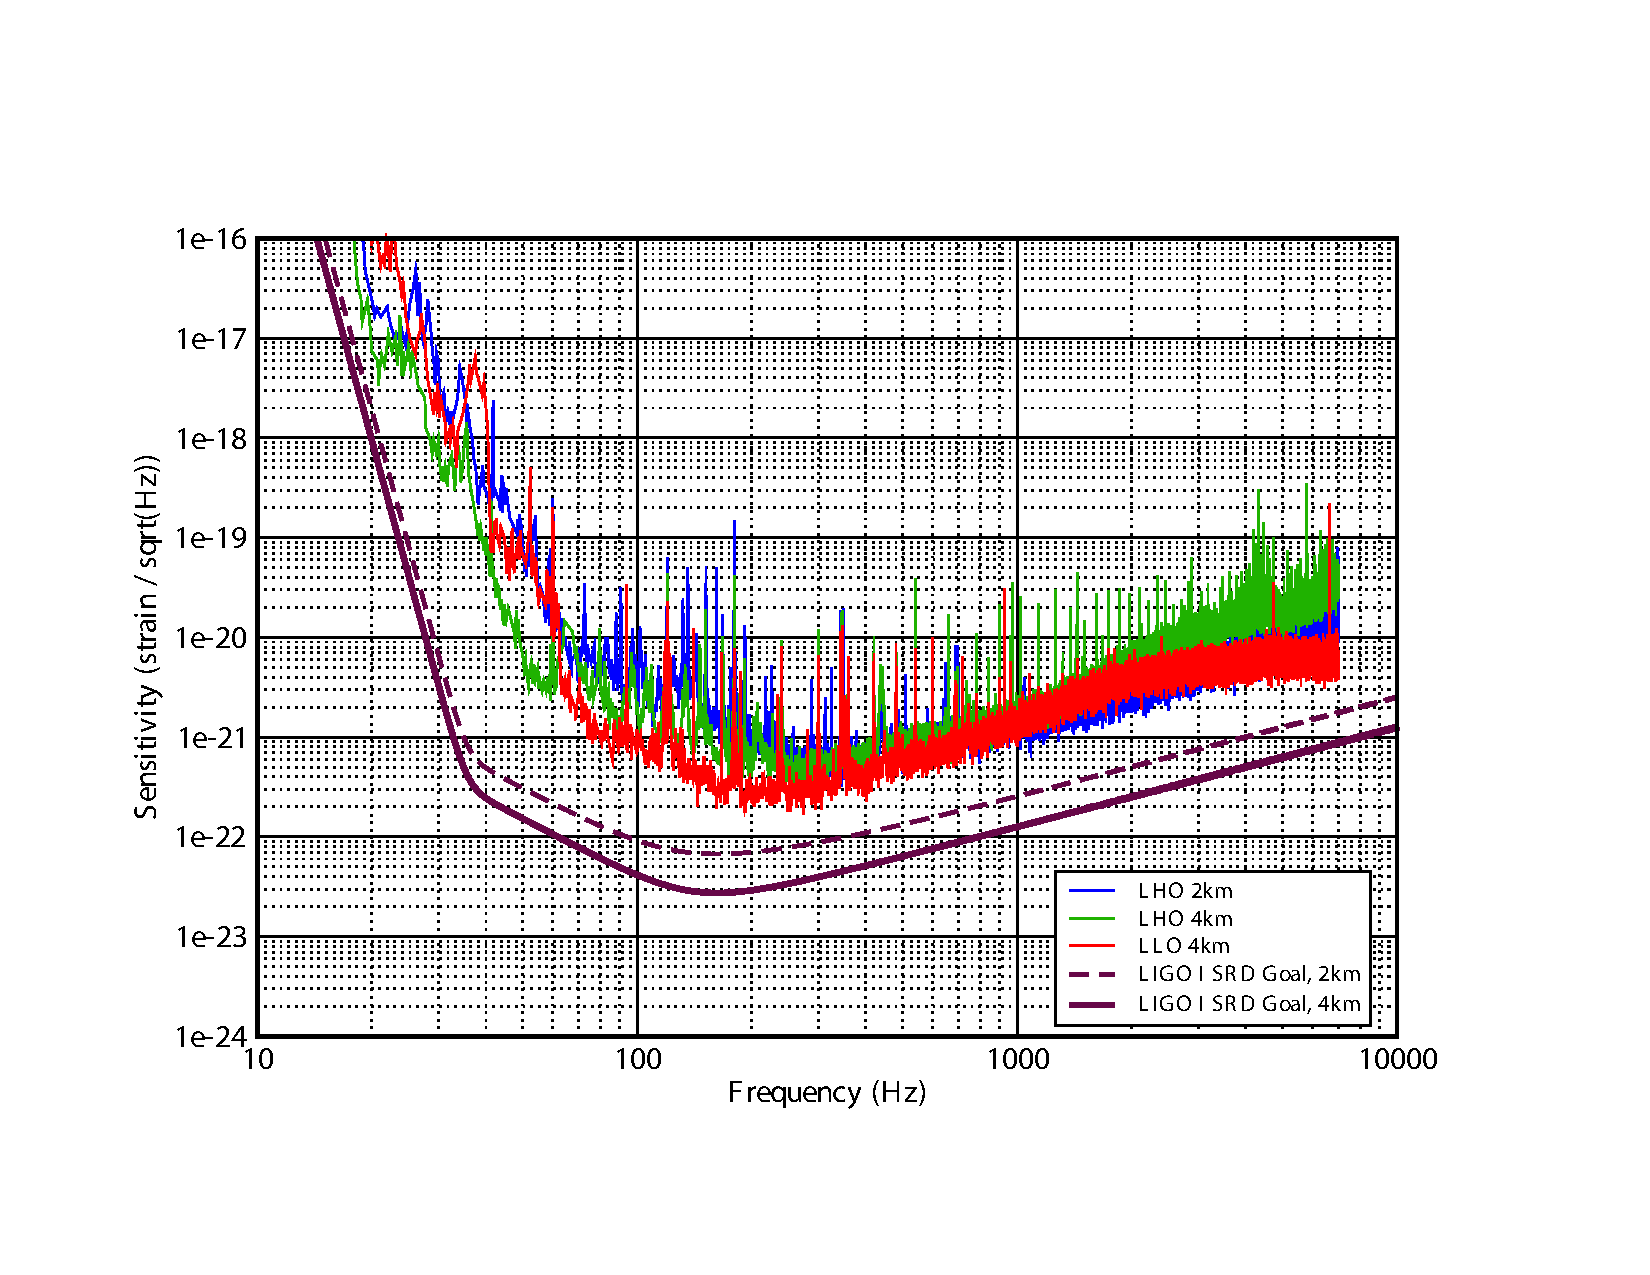
\includegraphics[width=\textwidth]{figures/pipeline/G030379-00}    
\end{center}
\caption{\label{f:s2noisecurve}%
Typical sensitivities of the three LIGO interferometers during the second LIGO
science run\cite{s2noisecurve} shown as strain amplitude spectral density,
$\tilde{h}/\sqrt{\mathrm{Hz}}$. The smooth solid curve shows the design
sensitivity (SRD Goal) of the $4$~km interferometers and the smooth dashed
curve shows the design sensitivity of the $2$~km interferometer.
}
\end{figure}

\begin{table}[p]
\begin{center}
\begin{tabular}{lcccccccc}
H1 Data Quality Cut      &$T\mathrm{total}$&$T_\mathrm{play}$&$T_\mathrm{done}$&$\rho>8$&$\rho>10$&$\rho>12$ \\
(1)                      &(2)     &(3)    &(4)    &(5)     &(6)     &(7)\\\hline
ASQ\_LOWBAND\_OUTLIER    &  14741 &  1990 &  1536 &   625  &  178   &   2 \\
ASQ\_OUTLIER\_CLUSTER    &  20407 &  1800 &  1800 &     0  &    0   &   0 \\
ASQ\_OUTLIER\_CORRELATED &   3126 &   558 &   456 &   390  &  167   &   2 \\
ASQ\_UPPERBAND\_OUTLIER  &  22817 &  1876 &  1876 & 15435  &10159   &7574 \\
AS\_PD\_SATURATION       &     72 &     5 &     0 &     0  &    0   &   0 \\
MICH\_FILT               & 118807 & 11400 & 11400 &  4443  & 3922   &3185 \\
\hline\hline
\\
H2 Data Quality Cut      &$T\mathrm{total}$&$T_\mathrm{play}$&$T_\mathrm{done}$&$\rho>8$&$\rho>10$&$\rho>12$ \\
(1)                      &(2)     &(3)    &(4)    &(5)     &(6)     &(7)  \\\hline
AS\_PD\_SATURATION        &    4   &   0   &   0  &    0  &    0   &   0 \\
MICH\_FILT                &64368   &6570   &5648  & 1294  &  164   &   7 \\
\hline\hline
\\
L1 Data Quality Cut      &$T\mathrm{total}$&$T_\mathrm{play}$&$T_\mathrm{done}$&$\rho>8$&$\rho>10$&$\rho>12$ \\
(1)                      &(2)     &(3)    &(4)    &(5)     &(6)     &(7)  \\\hline
ASQ\_LARGEP2P            &   2699 &   380 &     0  &    0 &    0  &    0 \\
ASQ\_OUTLIER\_CORRELATED &    840 &    60 &    60  &    0 &    0  &    0 \\
AS\_PD\_SATURATION       &    646 &    61 &    10  &  813 &  119  &    6 \\
MICH\_FILT               & 203539 & 21696 & 17794  & 6393 &  497  &   32 \\
NONSTAND\_CTRLS          &   4020 &   843 &    18  &    0 &    0  &    0 \\
\end{tabular}
\end{center}
\caption{\label{t:s2dqresults}%
The table shows the inspiral triggers generate from science mode data with the
mandatory data quality cuts applied. For each descretionary data quality cut
applied a given inteferometer (1), the amount of time that would be excluded
from the total science mode data by the cut is given (2). Since we tune data
quality cuts on playground data, the amount of playground time excluded is
also shown (3) and the amount of playground data analyzed for triggers (4).
These may differ for reasons explained in section \ref{ss:splitup}. The number
inspiral triggers generated when a particular data quality cut is active is
shown for different signal-to-noise thresholds (5--7). To generate the
triggers, interferometer data was high passed above $50$~Hz in the time domain
and a low frequency cutoff of $70$~Hz was applied to frequency domain.
Template banks were generated with a minimal match of $0.97$ and the
signal-to-noise threshold for the matched filter was set to $\rho_\ast = 8$. A
$\chi^2$ veto with $8$ bins applied with a threshold of $\chi^2 < 20 (8 +
0.03^2 \rho^2)$. 
}
\end{table}

\begin{table}[p]
\begin{center}
\begin{tabular}{ll}
Discretionary Data Quality Cut  & Applied \\\hline\hline
MICH\_FILT                 & No \\
\multicolumn{2}{l}{\parbox{\linewidth}{\footnotesize The cut would exclude a
large number of triggers, but would reduce the amount of data in the search
significantly. It was decided not to apply this cut and to try and exclude
false triggers from these times by a combination of coincidence, vetoes and
reducing the $\chi^2$ threshold.}}\\
\\
AS\_PD\_SATURATION        & Yes \\
\multicolumn{2}{l}{\parbox{\linewidth}{\footnotesize Clear correlation with
inspiral triggers with large signal-to-noise ratios in L1 and the study
described in section \ref{ss:photodiode} suggest that this should be used. The
lack of correlated trigger in H1 was due to the fact that the playground did
not sample any times with photodiode situations.\baselineskip=14pt}}\\
\\
ASQ\_LARGEP2P             & No \\
\multicolumn{2}{l}{\parbox{\linewidth}{\footnotesize A loud inspiral signal
could trigger this cut, so it is unsafe for use.\baselineskip=14pt}} \\
\\
NONSTAND\_CTRLS           & Yes \\
\multicolumn{2}{l}{\parbox{\linewidth}{\footnotesize Advice from experimental
team advised that detections made during this time could not be
trusted.\baselineskip=14pt}} \\
\\
ASQ\_OUTLIER\_CLUSTER     & No \\
\multicolumn{2}{l}{\parbox{\linewidth}{\footnotesize Gaby.\baselineskip=14pt}} \\
\\
ASQ\_OUTLIER\_CORRELATED  & No \\
\multicolumn{2}{l}{\parbox{\linewidth}{\footnotesize Gaby.\baselineskip=14pt}} \\
\\
ASQ\_LOWBAND\_OUTLIER     & No \\
\multicolumn{2}{l}{\parbox{\linewidth}{\footnotesize Gaby.\baselineskip=14pt}} \\
\\
ASQ\_UPPERBAND\_OUTLIER   & Yes \\
\multicolumn{2}{l}{\parbox{\linewidth}{\footnotesize Times with high upperband
noise in H1 are clearly correlated with high signal-to-noise ratio triggers.
In order to prevent the cut from begin triggered by real signals we also
require that the cut is on for more that $180$ seconds. The longest inspiral
signal in the S2 analysis is $52$ seconds.\baselineskip=14pt}}\\
\end{tabular}
\end{center}
\caption{\label{t:s2dqchoice}%
The final selection and justification of discretionary data quality cuts for
the S2 binary neutron star and binary black hole MACHO searches.}
\end{table}

\begin{figure}[p]
\begin{center}
\hspace*{-0.2in}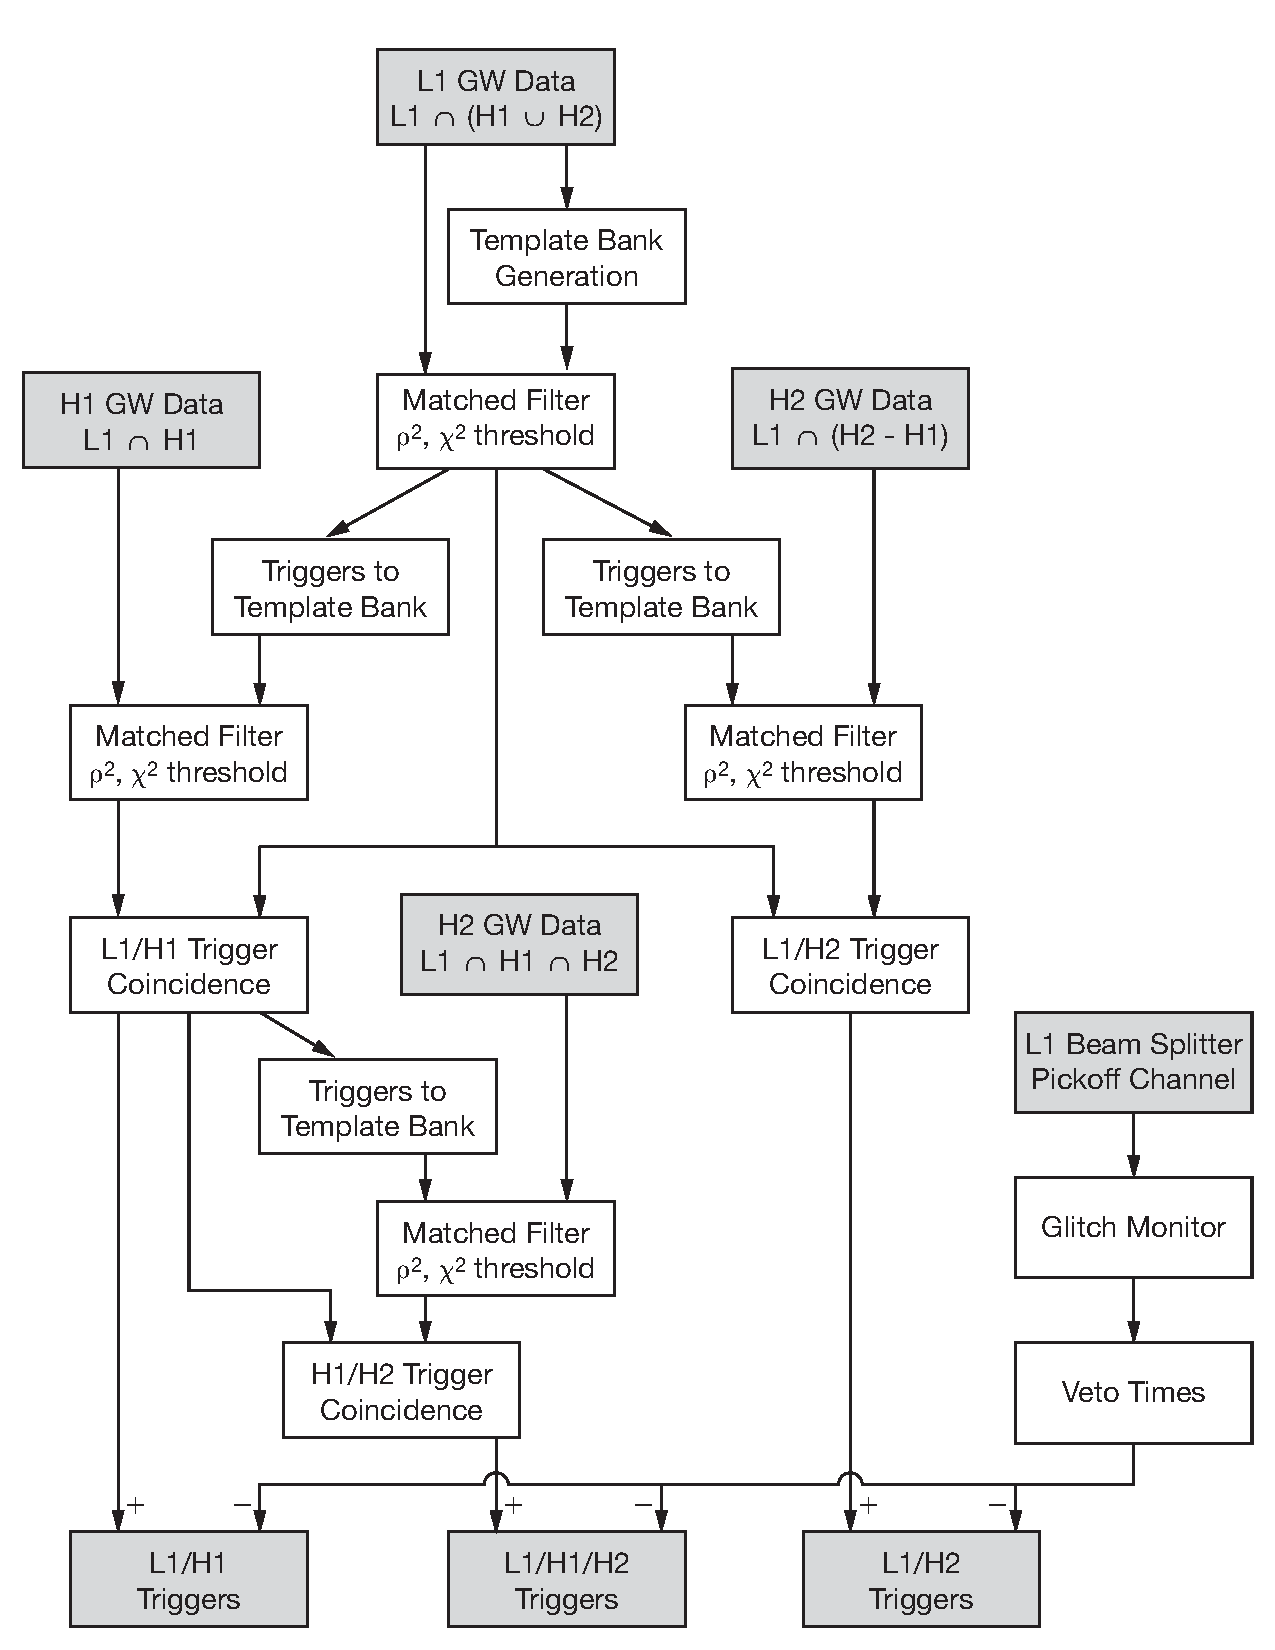
\includegraphics[width=0.6\textheight]{figures/pipeline/s2_pipeline}
\end{center}
\caption{\label{f:pipeline}%
The inspiral analysis pipeline used to determine the reported upper
limit. $\mathrm{L1} \cap (\mathrm{H1} \cup \mathrm{H2})$ indicates times when
the L1 interferometer was operating in coincidence with one or both of the
Hanford interferometers. $\mathrm{L1} \cap \mathrm{H1}$ indicates times when
the L1 interferometer was operating in coincidence with the H1 interferometer.
$\mathrm{L1} \cap (\mathrm{H2} - \mathrm{H1})$ indicates times when the L1
interferometer was operating in coincidence with only the H2 interferometer.
The outputs of the search pipeline are triggers that belong to one of the
two double coincident data sets or to the triple coincident data set.}
\end{figure}

